\documentclass{beamer}


\usepackage[utf8]{inputenc}
\usepackage{xcolor}
\usepackage[framemethod=tikz]{mdframed}
\usepackage{tcolorbox}
\usepackage[activate={true,nocompatibility},final,tracking=true,kerning=true,spacing=true,factor=1100,stretch=10,shrink=10,expansion]{microtype}
\SetTracking{encoding={*}, shape=sc}{0}
\usepackage{pifont}
\usepackage{graphics}
\usepackage[alf]{abntex2cite}



\usetheme{Malmoe}
\usecolortheme{wolverine}


\mode<presentation>


\title[LISTA 3]{\Huge{\textcolor{blue!70!black}{LISTA 3}}}

\author[Cassinha]{\textcolor{blue!70!black}{\huge{Maxuel Ribeiro Cassinha}}\\
\text{\scriptsize{\textcolor{blue!70!black}{maxuel.cassinha@usp.com.br}}}}

\date[EEL-USP]{\scriptsize{\textcolor{blue!70!black}{Mini-curso de \LaTeX}} \\ \textcolor{blue!70!black}{Universidade de São Paulo - LABEEL}}



%%%%%% ~~~~~~~~~ %%%%%%%%

%%%%%%%%%%% Começo do Corpo do Documento %%%%%%%%%%%%%%%%

%%%%%% ~~~~~~~~~ %%%%%%%%


\begin{document}

%{\usebackgroundtemplate{
\includegraphics[width=\paperwidth]{Imagens/TP.jpg}}}

  \begin{frame}
    \titlepage
  \end{frame}


\begin{frame}
  \frametitle{CAIXA}

\begin{tcolorbox}[colback=blue!70!white,colframe=blue!70!white,title=PAZ NA TERRA]
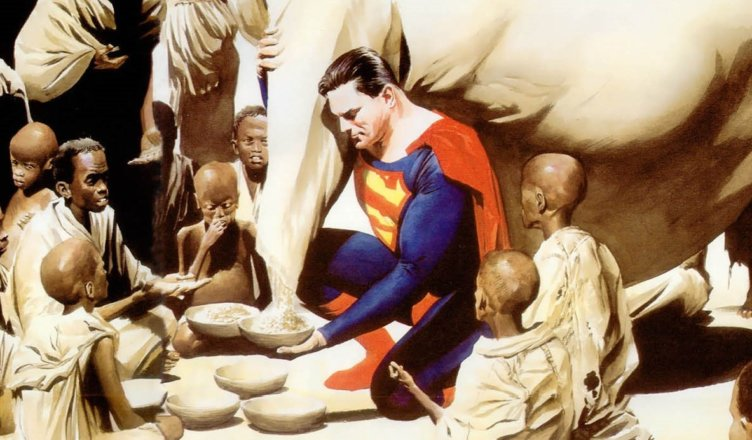
\includegraphics[width=0.8\paperwidth,height=0.7\paperheight]{Imagens/Paznaterra.jpg}

\end{tcolorbox}

\end{frame}

\begin{frame}
  \frametitle{Citação}
\begin{itemize}
    \item {\ding{170} \textcolor{blue!70!black}{"Relógio ou coração, o problema é o mesmo: ouvir se bate, perceber a que corpo dá vida"}}
    \item{\ding{166} \textcolor{blue!70!black}{\cite{pessoa2015melhores}}}
\end{itemize}

\end{frame}

\textcolor{blue!70!black}{\bibliography{ref-bib.bib}}

\end{document}




%%% Local Variables:
%%% mode: latex
%%% TeX-master: t
%%% End:
